% !TEX spellcheck = en_US

\documentclass[conference]{IEEEtran}
\usepackage{cite}
\usepackage{amsmath,amssymb,amsfonts}
\usepackage{algorithmic}
\usepackage{graphicx}
\usepackage{textcomp}
\usepackage{xcolor}
% add hyperlinks, delete all .aux files if adding hyperref after previous build
\usepackage{hyperref}
% support for unicode charcters like "é" and "ñ"
\usepackage[T1]{fontenc}
% Provides generic commands \degree, \celsius, \perthousand, \micro and \ohm
\usepackage{gensymb}
% splits a section into multiple columns
\usepackage{multicol}
\usepackage{balance}
% balance columns on lastpage
% better than \flushend according to
% https://texfaq.org/FAQ-balance
%\usepackage{flushend}

\def\BibTeX{{\rm B\kern-.05em{\sc i\kern-.025em b}\kern-.08em
    T\kern-.1667em\lower.7ex\hbox{E}\kern-.125emX}}
\begin{document}

\title{Effects of Solar Resource Sampling Rate and Averaging Interval on Hourly Modeling Errors}

\author{\IEEEauthorblockN{Mark A. Mikofski, William F. Holmgren, Jeffrey Newmiller, and Rounak Kharait}
\IEEEauthorblockA{DNV, Oakland, CA, 94612, USA }}

\maketitle

\begin{abstract}
Solar energy modeling errors due to time-averaged hourly inputs are significant where solar resource variability and inverter loading ratio are both high. However, predictions of PV system performance are most frequently made with hourly solar resource inputs, typically computed from satellite data obtained every 15 or 30 minutes. Therefore, we studied the effects of solar resource sampling rate and time-averaging interval on hourly modeling errors by using high frequency measurements from 8 different locations across the United States. When we selected minute-average measurements at various sampling rates and averaged them to hourly data, we observed increasing modeling errors for sampling rates 30-minutes or shorter. At a 30-minute sampling rate averaged hourly we observed an error that was 50\% of 1-minute samples averaged hourly. As sampling rate approached 60 minutes, modeling errors decreased, partially canceling out due to the randomness of the low frequency sampled data. We examined PV systems with DC/AC > 1.3 and observed that clipping errors dominated modeling errors from other sources like transposition to plane-of-array irradiance at sites with greater solar variability. Based on our analysis, we recommend that an hourly modeling correction be applied whenever hourly inputs are used, especially at sites with high solar variability and DC/AC ratios greater than one.
\end{abstract}

\begin{IEEEkeywords}
inverter, clipping, satellite, sampling, solar resource, irradiance, variability, performance, modeling, TMY
\end{IEEEkeywords}

\section{Introduction}
Accurate solar energy assessments are important for lowering the cost of capital for PV systems. However, continuing under-performance of solar assets over the past few years may be damaging investor confidence \cite{Matsui2021}. Several studies have examined potential sources of under-prediction, and modeling errors due to hourly inputs have recently received renewed interest \cite{Parikh2021,Anderson2020,Bradford2020,Kharait2020,Cormode2019}. These modeling errors arise from differences in predicted power production between using hourly versus subhourly input, due to various non-linear mechanisms including notably inverter maximum power clipping and irradiance transposition. When hourly input is time-averaged from \emph{high} frequency subhourly weather measurements, energy output is over-predicted and clipping losses are under-predicted. However, most energy assessments typically use satellite data which is averaged hourly from \emph{low} frequency measurements sampled at 15-minute or 30-minute intervals \cite{Wilcox2012,Sengupta2018}. Recently, a few studies have investigated the difference between hourly input time-averaged from high frequency versus hourly input generated from low frequency sampled data and have demonstrated that modeling errors appear to be reduced for slower sampled data \cite{Bowersox2021,osti_1797569}. Ideally, high frequency data would be used for all modeling stages, but in practice the data have been time-averaged from low frequency samples, and this time averaging is itself a source of discrepancies between modeled and measured performance. This study examines the impact of solar resource sampling rate on hourly PV modeling error using high frequency ground irradiance measurements at the NIST ground array \cite{Boyd2017,Boyd2017a,Boyd2017b} and the 7 SURFRAD stations \cite{Augustine2000}. In the following sections we describe our methods, show our results, and discuss our observations. By analyzing the effect of sampling rate and time averaging from the same underlying dataset of high quality ground measurements, we side-step any additional modeling discrepancies that might result, for instance, from differing spatial resolution between ground and satellite measurements, or algorithms used to estimate solar irradiance from satellite image properties. This study is thus a direct examination of the effects of time averaging and sampling frequency isolated from other sources of error.

\section{Methods}

\subsection{NIST Ground Array Configuration}
For the first part of this study, we used a model of the NIST ground array, a fixed-tilt 260-kW PV system \cite{Boyd2017,Boyd2017a,Boyd2017b}, as the base system and simulated varying the inverter loading ratio by adding additional DC capacity with the same pitch and racking as the existing rows to the model. A weather station at the site collects inputs at 1-minute frequency, allowing sampling of irradiance data at various rates by decimation of the recorded data. SolarFarmer \cite{solarfarmer2018} can use inputs at any frequency, so it was used to simulate a fictitious version of the NIST ground array with a DC/AC ratio of 1.5. Simulated AC power output from SolarFarmer has the same frequency as the input weather data, and both are assumed to represent the average during that interval. For example, if the input is every 5-minutes, then the output is also every 5-minutes and assumed to be constant during that 5-minute interval.

\subsection{Generic Array Configuration for SURFRAD}
For the second part of this study, we simulated a system consisting of strings of generic 300-W mono-crystalline silicon modules (Canadian Solar CS6X-300M) connected to a single generic 250kW central inverter (SMA America SC250U (480V)), such that the DC/AC ratio was 1.3. The module and inverter parameters were sourced from the NREL System Advisor Model (SAM) libraries \cite{Freeman2018}. There are 7 SURFRAD \cite{Augustine2000} stations across the United States, listed in Table \ref{table:SURFRAD-summary}, that provide 1-minute average input since 2009. Compared to hourly irradiance data, 1-minute is relatively ``instantaneous''. Therefore, we refer to the SURFRAD 1-minute averages as instantaneous for the remainder of this paper. The instantaneous data was used with pvlib python \cite{pvlib2018} to predict plane-of-array (POA) irradiance components, effective irradiance, cell temperature, DC power, and AC output. The method was based on a previous study \cite{9519024} with minor differences. SURFRAD data was filtered for data quality, visually inspected, and problematic rows were dropped from the dataset. Then, only years containing at least 98\% of global horizontal irradiance (GHI), diffuse horizontal irradiance (DHI), direct normal irradiance (DNI), air temperature, wind speed, relative humidity, pressure, and solar zenith were considered. The SURFRAD irradiance components were checked for self consistency. The analysis is available from GitHub here: \url{https://github.com/mikofski/pvsc49-satellite-sampling}.

Wind speed measurements were available so the thermal coefficients were changed to $U_c=25, U_v=1.2$, and a moving average with a 10-minute window was used to smooth unrealistic high frequency cell temperatures \cite{9095219}. Finally the Sandia National Laboratory performance model for grid-connected PV inverters \cite{King2007} was used to calculate AC power ($E_{grid}$).

\subsection{Input Data}
This study uses a method similar to others to time-average low frequency sampled irradiance data from higher frequency measurements \cite{Bowersox2021,osti_1797569} as a proxy for satellite-derived data. By using time-averaged or decimated samples from the same ground dataset, the model results show directly the differences in energy output that are attributable to time-averaging or lower sampling frequency that are typically featured in satellite datasets. Using each full year of data from each of the 8 locations, we created 15 different sets of irradiance input from the 1-minute measurements to study the effect of sampling rate and time averaging on the modeling error. The datasets can be grouped into three categories: \emph{time-averaged}, \emph{instantaneous}, and \emph{simulated hourly satellite} each with 5 datasets that have either time-averaged or instantaneously sampled data at the following intervals or frequencies:

\begin{itemize}
    \item 1-minute
    \item 5-minutes
    \item 15-minutes
    \item 30-minutes
    \item 60-minutes
\end{itemize}

\emph{Time-averaged}: The first 5 datasets are the 1 minute records time-averaged at the different intervals. We do this to simulate the modeling error observed when high frequency input data is averaged.

\emph{Instantaneous}: The next 5 datasets were generated by selecting (decimating) 1-minute records from the onsite measurements. For example, to generate the 15-minute sampled data from the NIST weather station 4 records per hour were selected at the 7th, 22nd, 37th, and 52nd minutes as shown in Fig.~\ref{fig:sampling-diagram}. For the 7 SURFRAD sites the 1st, 16th, 31st, and 46th minutes were selected to generate the 15-minute instantaneous dataset. Also note that both the 1-minute time-averaged and instantaneous datasets are actually identical, because 1-minute was the resolution of the measured data.

\emph{Simulated hourly satellite}: The last 5 datasets time-average the records in the instantaneous datasets to 1-hour as a proxy for satellite-derived irradiance data. For example, to generate the 15-minute simulated ``satellite'' data from the NIST weather station, the 4 records shown in Fig.~\ref{fig:sampling-diagram} were averaged together to create one value for that hour. Note that the 60-minute time-averaged and 1-minute simulated ``satellite'' datasets are also identical because they both aggregate the 1-minute measured data to hourly. Also note that all of the simulated ``satellite'' data provide hourly inputs to the performance model, while the time-averaged and instantaneous inputs have the resolutions given by the time-averaging interval or the instantaneous sampling rate.

\begin{figure}[htbp]
\centerline{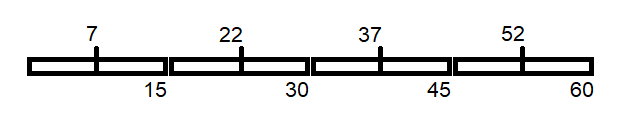
\includegraphics[width=9cm]{sampling-diagram.png}}
\caption{This diagram demonstrates how records were selected to generate 15-minute sampled datasets from the NIST weather station by selecting only 4 records at the 7th, 22nd, 37th, and 52nd minutes. Then to simulate ``satellite'' data, these 4 instantaneous records were averaged together to create a single value for the hour.}
\label{fig:sampling-diagram}
\end{figure}

\subsection{Metrics}
The simulated hourly ``satellite'' datasets are representative of the time-averaged information that is typically available for input to energy production simulation software. The model outputs derived from these datasets serve as the typical modeling results (reference) that will require correction to improve accuracy, but the remaining analysis focuses on deviation relative to the ``best fidelity'' model simulated directly from the 1-minute instantaneous data.

\begin{equation} \label{eq:1}
E_e = \frac{E_\mathrm{grid,clipped,dataset}}{E_\mathrm{grid,clipped,1\text{-}min}} - 1
\end{equation}

\begin{equation} \label{eq:2}
\mathit{CL} = \frac{E_\mathrm{grid,clipped,dataset}}{E_\mathrm{grid,unclipped,dataset}} - 1
\end{equation}

That is, the modeling error ($E_e$) is quoted relative to the best fidelity result as given by Eqn.~\ref{eq:1}, and the clipping loss ($\mathit{CL}$) is relative to the unclipped output of the same dataset as given by Eqn.~\ref{eq:2}.

\section{Results}
\label{section:results}

\subsection{Analysis of NIST Ground Array}
The annual energy yield, POA irradiance, and as-modeled clipping losses for each of the 15 SolarFarmer predictions for the NIST ground array are shown in Table~\ref{table:results-summary}. Clipping loss ($\mathit{CL}$) is defined in Eqn.~\ref{eq:2} as the fraction of energy clipped relative to the output if there were no clipping, where clipping refers to power that is not generated because it is greater than the inverter rating during an as-simulated time interval. Depending on the dataset, the 2nd column shows either the sampling rate or the averaging interval. The rows in the first section show the results from the \emph{time-averaged} dataset in which 1-minute input is time-averaged at different intervals. The rows in the second section show results from the \emph{instantaneous} dataset in which input is sampled at different rates. The rows in the third section show results from the \emph{simulated satellite} dataset in which instantaneous data was averaged to hourly. Note that the 1-minute \emph{time-averaged} results are identical to the 1-minute \emph{instantaneous} results, because the NIST resource data resolution is 1-minute and all modeling follows that resolution in both cases. Also note that the 60-minute \emph{instantaneous} results are identical to the 60-minute \emph{simulated satellite} results because both were obtained from an hourly sampling rate. Finally, the 60-minute \emph{time-averaged} results are the same as the 1-minute \emph{simulated satellite} results because both model results every minute and average hourly.

\begin{table}[htbp]
\caption{SolarFarmer Annual Results for NIST Ground Array}
\begin{center}
\begin{tabular}{|c|c|c|c|c|}
\hline
\textbf{Dataset} & \textbf{\textit{Rate | Interval}} & \textbf{\textit{Energy Yield}} & \textbf{\textit{POA}} & \textbf{\textit{Clipping}} \\
& \textit{minutes} & \textit{kWh/kWp} & \textit{kWh/m\textsuperscript{2}} & \textbf{\textit{Loss}} \\
\hline
             &  1& 1286.3& 1667.4& -4.6\% \\
time-        &  5& 1298.3& 1669.2& -4.2\% \\
averaged     & 15& 1308.7& 1671  & -3.9\% \\
(interval)   & 30& 1314.8& 1672  & -3.8\% \\
             & 60& 1320.8& 1673.5& -3.5\% \\
\hline
             &  1& 1286.3& 1667.4& -4.6\% \\
instant      &  5& 1285.9& 1667.7& -4.6\% \\
(rate)       & 15& 1285.4& 1668.2& -4.6\% \\
             & 30& 1285.6& 1665.1& -4.5\% \\
             & 60& 1284  & 1663.1& -4.5\% \\
\hline
             &  1& 1320.8& 1673.5& -3.5\% \\
simulated-   &  5& 1319.3& 1673.6& -3.6\% \\
satellite    & 15& 1315  & 1673.8& -3.7\% \\
(rate)       & 30& 1304.9& 1669  & -3.9\% \\
             & 60& 1284  & 1663.1& -4.5\% \\
\hline
\end{tabular}
\label{table:results-summary}
\end{center}
\end{table}

The 1-minute time-averaged input, shown in the first row, correctly accounts for rapid ramp rates in the solar resource when predicting energy yield, POA irradiance, and clipping loss. As the time-averaging interval increases to hourly, the energy yield is over-predicted by 2.7\%, the clipping loss is under-predicted by absolute delta of 1.1\% , and the POA irradiance is also over-predicted by 0.4\% relative to the 1-minute measurements. The data in the last 3 columns of Table~\ref{table:results-summary} are plotted in Fig.~\ref{fig:NIST-energy-yield}, ~\ref{fig:NIST-clipping-loss}, \& ~\ref{fig:NIST-POA}, to help visualize how the model output changes versus sampling rate or averaging interval of the input from each dataset.

Fig.~\ref{fig:NIST-energy-yield} shows a plot of the time-averaged, instantaneous, and simulated ``satellite'' energy yield. The 1-minute \emph{time-averaged} input/compute-interval accounts for rapid ramp rates in solar resource with best available fidelity for this data. As the input is time-averaged over longer intervals, the energy yield is over-predicted, with the largest changes occurring from 1-minute to 15-minute time-averaging intervals. As input data is sampled at lower frequency, random errors occur in the input data and cancel out the modeling error. For example, instantaneous sampling every 30 minutes yields input randomly greater or less than the average during the same time-interval.

The \emph{simulated satellite} 1-minute results are identical to the 60-minute \emph{time-averaged}, because they both show 1-minute measurements averaged hourly. Therefore, as input data is sampled at increasing frequency approaching 1-minute sampling and averaged hourly, the modeling errors ($E_e$) increase and approach the same as 60-minute \emph{time-averaged}. All of the \emph{simulated satellite} input is averaged hourly, so this trend is similar but opposite to the increase in modeling errors observed in \emph{time-averaged} input as the interval is increased. The inflection point seems to be around 30-minutes. At sampling times longer than 30-minutes, random errors occur in the input data and roughly cancel the modeling error, similar to observations of the \emph{instantaneous} results. However, we observe that even for input data sampled every 30-minutes, similar to the sampling rate of NSRDB TMY3 files, there is still non-zero modeling error.

\begin{figure}[htbp]
\centerline{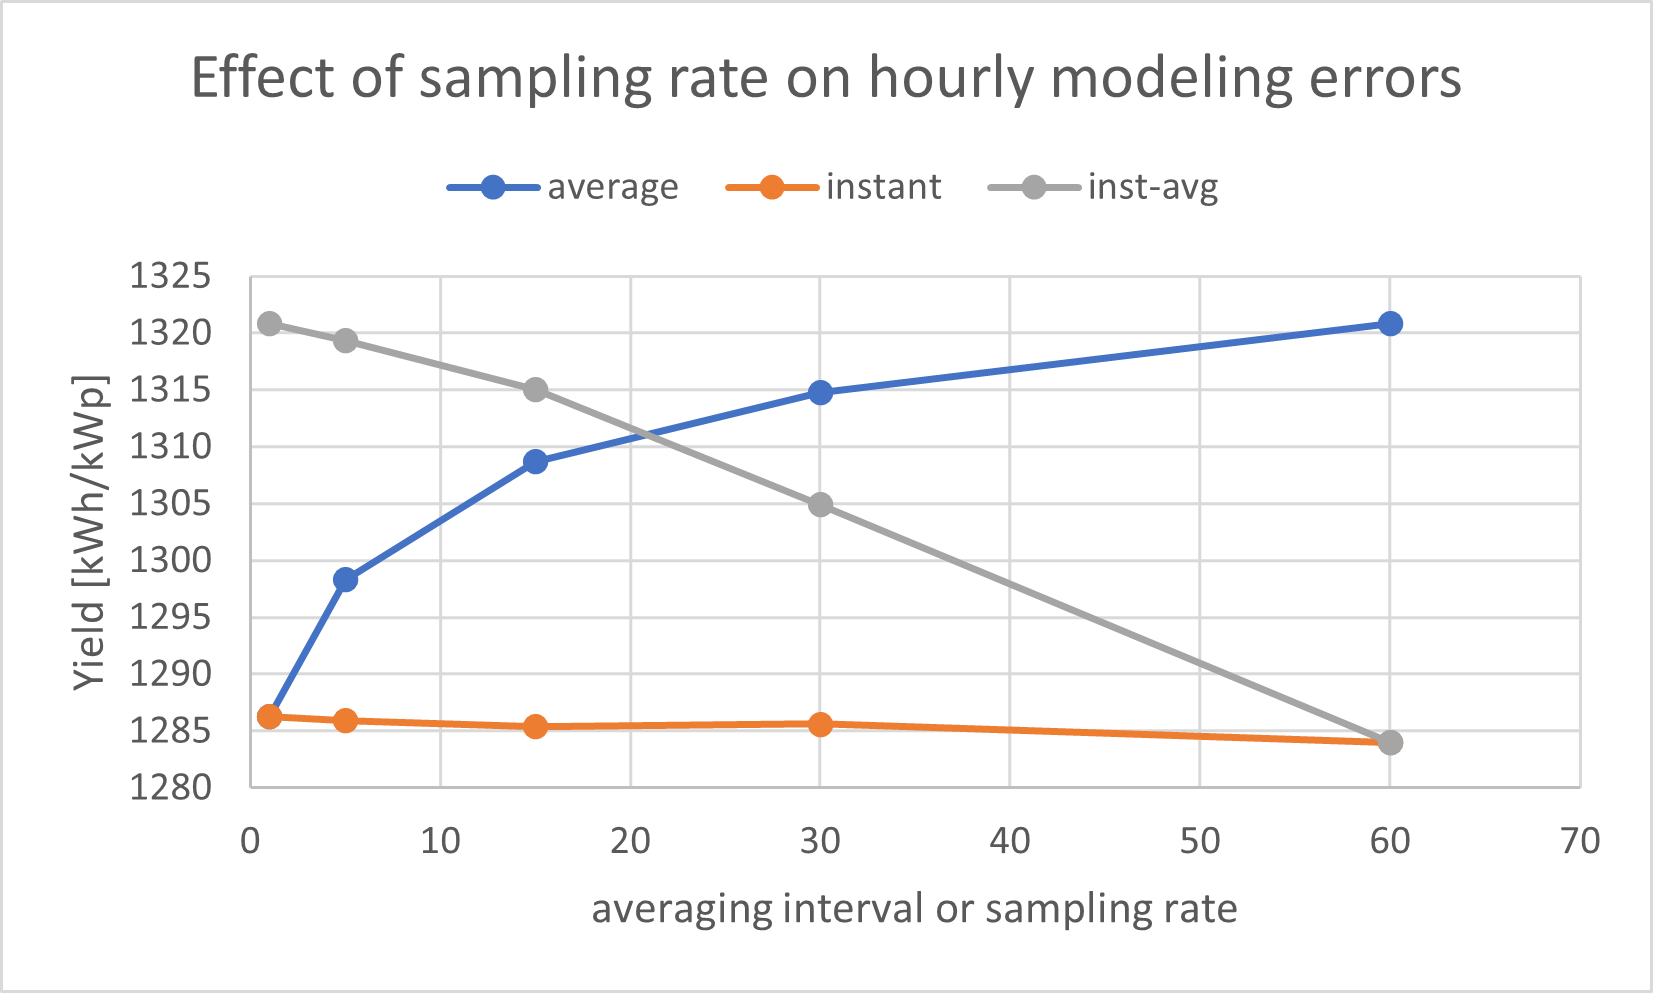
\includegraphics[width=9cm]{NIST_energy_yield.png}}
\caption{Energy yield for all 3 datasets shows over-prediction relative to 1-minute if time-averaged to 60-minutes. Simulated ``satellite'' (inst-avg) has non-zero errors at 30-minute sampling rates and increasing errors for shorter sampling rates. Instantaneous has random errors that cancel out.}
\label{fig:NIST-energy-yield}
\end{figure}

\begin{figure}[htbp]
\centerline{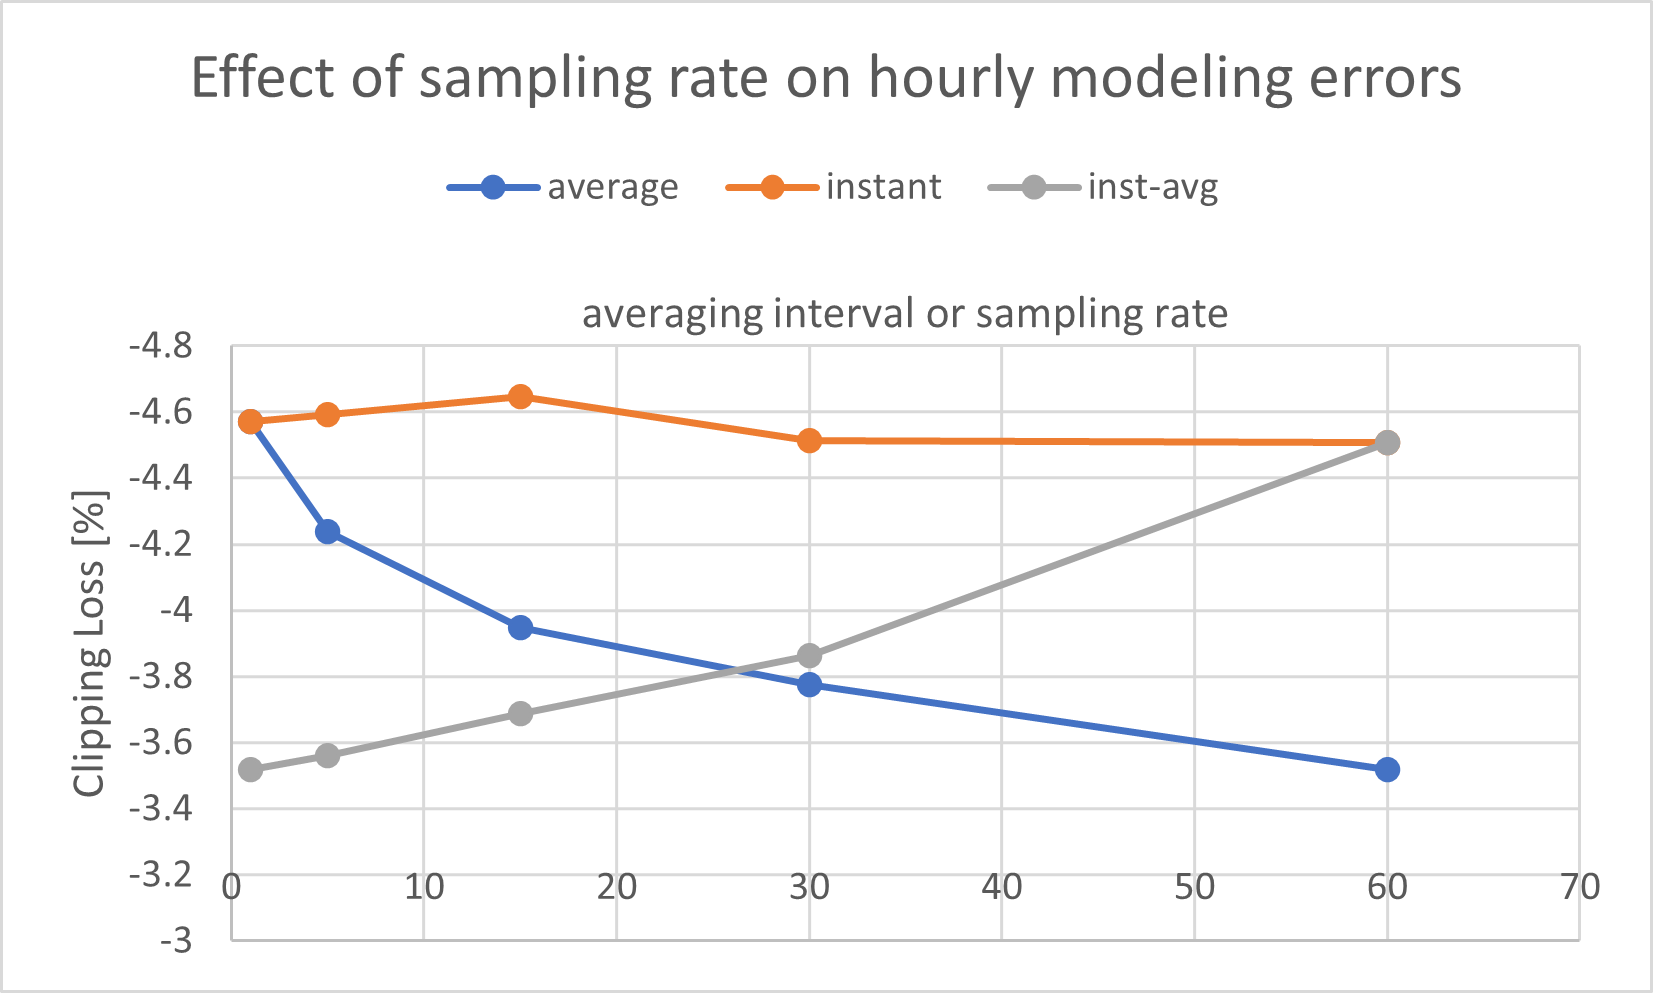
\includegraphics[width=9cm]{NIST_clipping_loss.png}}
\caption{Clipping losses for all 3 datasets shows under-prediction relative to 1-minute if time-averaged to 60-minutes. Simulated ``satellite'' (inst-avg) has non-zero errors at 30-minute sampling rate and increasing errors for shorter sampling rates. Instantaneous has random errors that cancel out.}
\label{fig:NIST-clipping-loss}
\end{figure}

\begin{figure}[htbp]
\centerline{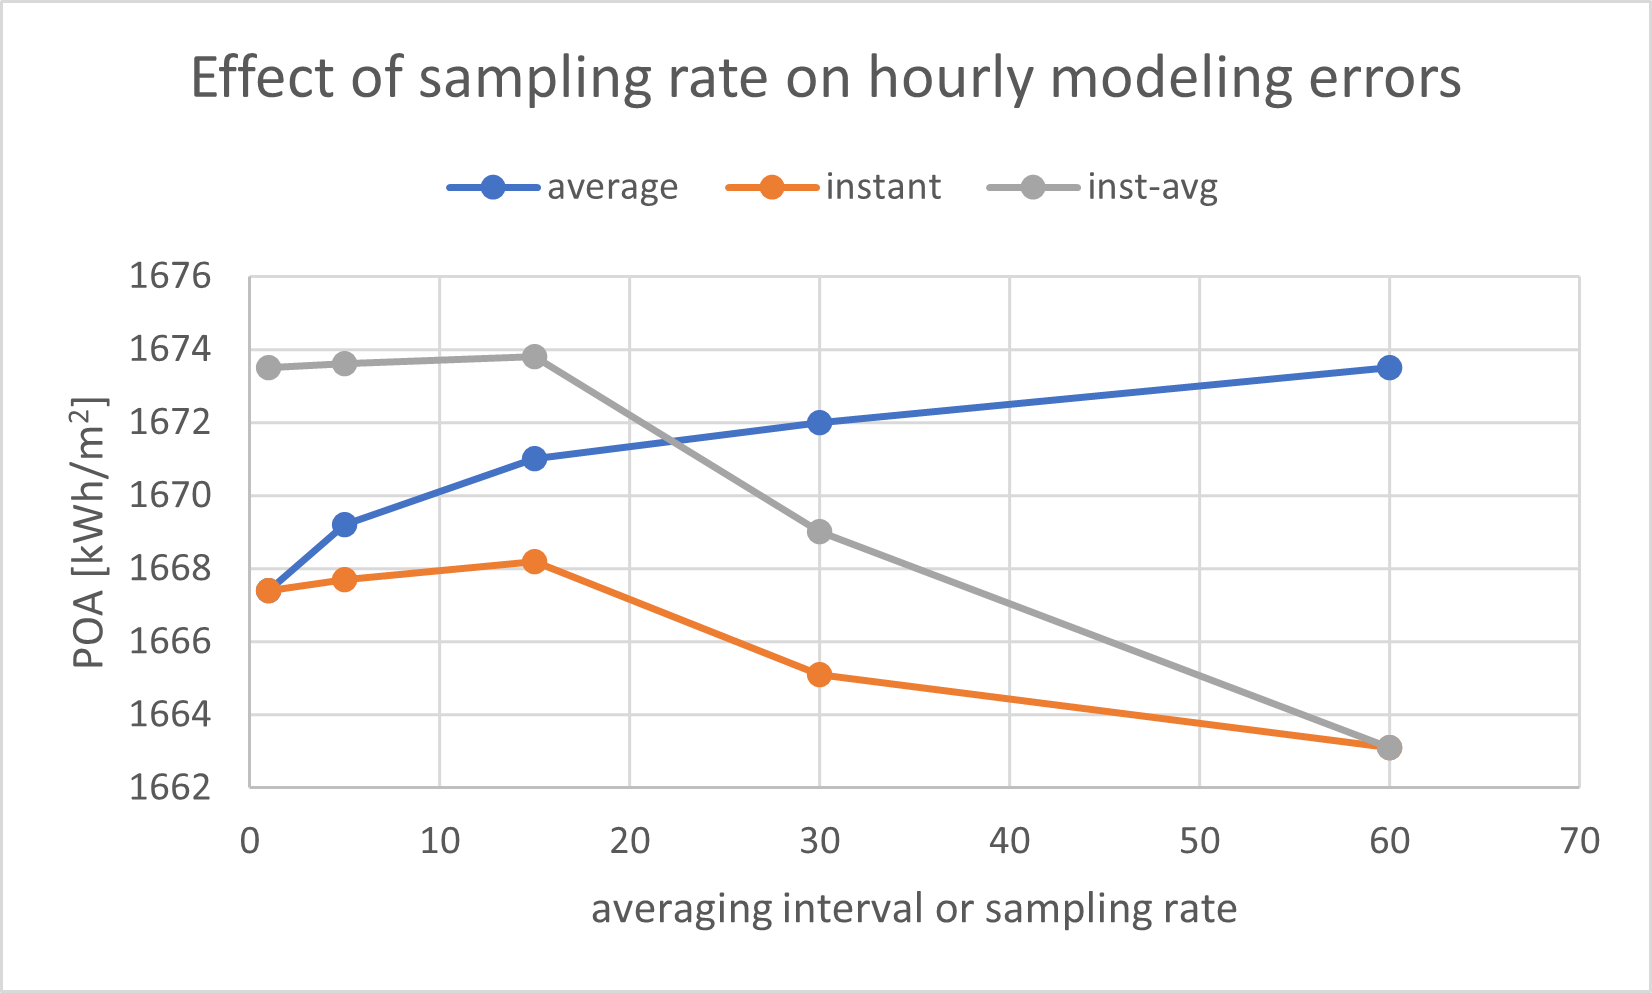
\includegraphics[width=9cm]{NIST_POA.png}}
\caption{POA irradiance for all 3 datasets shows significantly smaller errors compared to energy yield, implying that clipping errors dominate modeling errors due to hourly input for this particular scenario with DC/AC of 1.5. For lower DC/AC ratio, clipping errors will dominate less, and POA irradiance errors may become more significant.}
\label{fig:NIST-POA}
\end{figure}

Clipping losses for all 3 datasets are shown in Fig.~\ref{fig:NIST-clipping-loss}. Clipping losses are the percentage of AC power that is lost due to clipping. One should not compare modeling error between simulations based \emph{only} on clipping loss, because the delta in clipping losses is not equal to the modeling error. For example, the modeling error due to time-averaged hourly input was 2.7\% while the clipping losses only changed by absolute delta of 1.1\%. The modeling error due to hourly inputs is only defined by the change in AC power relative to 1-minute input. However, the clipping loss is useful in determining that clipping errors are the cause of the over-prediction in energy yield, for this particular scenario with DC/AC of 1.5. Lower DC/AC will have lower clipping losses, and therefore less modeling error due to clipping errors.

The POA irradiance, shown Fig.~\ref{fig:NIST-POA}, is also over-predicted when using hourly time-averaged inputs relative to 1-minute. However, the POA irradiance error is only 0.4\%, significantly less than the modeling error in energy yield. Therefore, we observe that clipping errors dominate the hourly modeling error, for this particular scenario with a DC/AC ratio of 1.5. For a lower DC/AC ratio, clipping errors will play a smaller role in energy yield, and POA irradiance errors may become more significant.

\subsection{Analysis of Generic Array with SURFRAD}
Annual modeling errors predicted for the generic array with pvlib python for each of the 15 datasets for each of the 7 SURFRAD stations are shown in Fig.~\ref{fig:bon2010}, \ref{fig:dra2011}, \ref{fig:fpk2009}, \ref{fig:gwn2012}, \ref{fig:psu2010}, \ref{fig:sxf2009}, \& \ref{fig:tbl2010}. The annual modeling errors for hourly averaged input and for simulated ``satellite'' with 30-minute sampling rate both relative to 1-minute are summarized in Table \ref{table:SURFRAD-summary} for all years.

\begin{table}[htbp]
\caption{Modeling Errors for SURFRAD Generic Arrays with pvlib}
\begin{center}
\begin{tabular}{|c|c|c|c|c|}
\hline
& & \multicolumn{2}{c|}{\textbf{\textit{Model Errors}}} & \\\cline{3-4}
\textbf{Station}& \textbf{\textit{Years}}& \textbf{\textit{60-min}} & \textbf{\textit{30-min}} & \textbf{\textit{Fraction}} \\
& & \textbf{\textit{averaged}} & \textbf{\textit{``satellite''}} &                                \\
\hline
Bondville, IL      & 8 & 2.1\% & 1.2\% & 59\% \\
Desert Rock, NV    & 9 & 0.95\%& 0.29\%& 30\% \\
Fort Peck, MT      & 6 & 1.9\% & 1.0\% & 53\% \\
Goodwin Creek, MS  & 1 & 1.3\% & 0.32\%& 24\% \\
Penn State, PA     & 5 & 2.4\% & 1.2\% & 51\% \\
Sioux Falls, SD    & 8 & 1.8\% & 1.1\% & 61\% \\
Boulder, CO        & 7 & 2.6\% & 2.0\% & 77\% \\
\hline
Summary& 44& 1.9\% & 1.0\% & 51\% \\
\hline
\end{tabular}
\label{table:SURFRAD-summary}
\end{center}
\end{table}

\begin{figure}[htbp]
\centerline{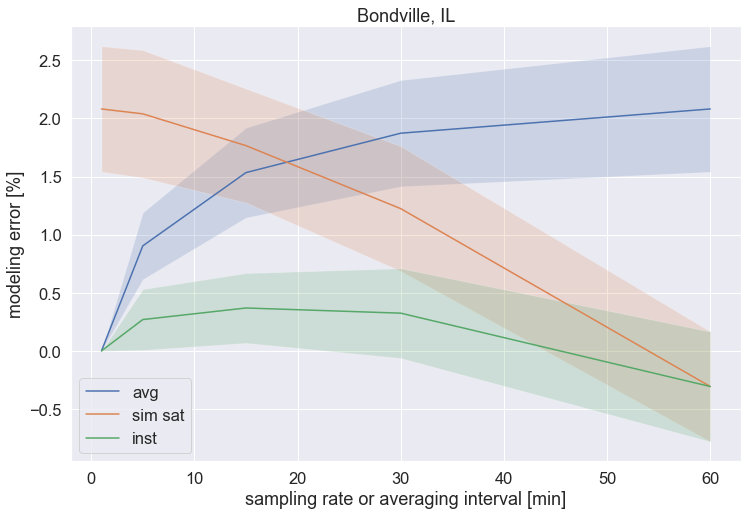
\includegraphics[width=9cm]{analysis/bon_all.png}}
\caption{Annual AC energy modeling error at Bondville, IL. The solid lines and shaded areas show the average and 1-$\sigma$. Time-averaged input (blue) increases with longer averaging interval, simulated ``satellite'' (red) decreases with slower sampling rate, while instantaneous (green) is relatively unchanged.}
\label{fig:bon2010}
\end{figure}

\begin{figure}[htbp]
\centerline{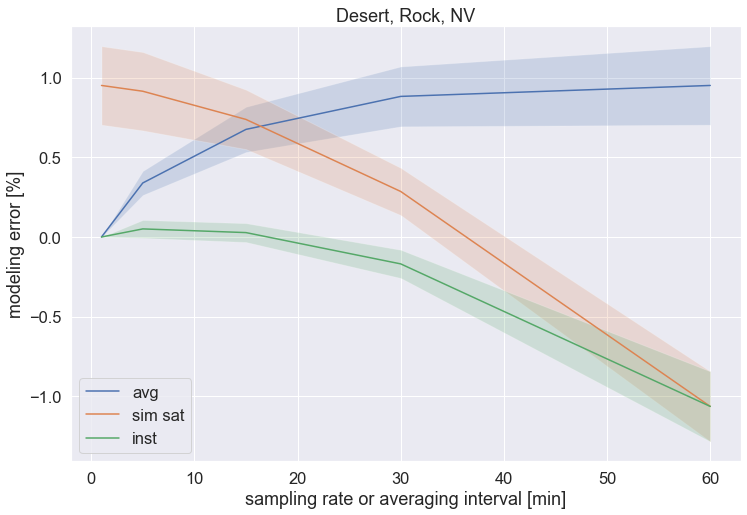
\includegraphics[width=9cm]{analysis/dra_all.png}}
\caption{Annual AC energy modeling error at Desert Rock, NV. The solid lines and shaded areas show the average and 1-$\sigma$. Desert Rock had the highest output and the lowest modeling error of the 7 SURFRAD sites presumably due to its high irradiance and clear skies. Negative model error at 60-minute instantaneous sampling rate (high-fidelity estimate greater than hourly estimate) may indicate an asymmetric distribution of irradiance at or below the hourly average.}
\label{fig:dra2011}
\end{figure}

\begin{figure}[htbp]
\centerline{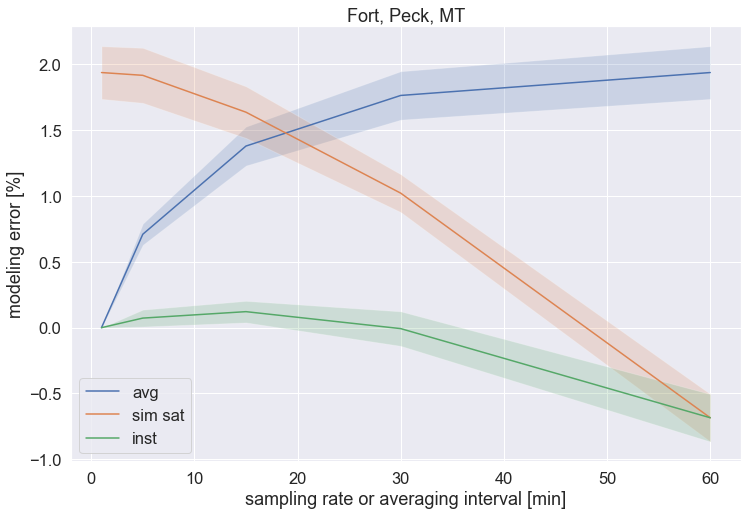
\includegraphics[width=9cm]{analysis/fpk_all.png}}
\caption{Annual AC energy modeling error at Fort Peck, MT. The solid lines and shaded areas show the average and 1-$\sigma$. Time-averaged input (blue) increases with longer averaging interval, simulated satellite (red) decreases with slower sampling rate, while instantaneous (green) is slightly negative at 60-minute instantaneous but relatively unchanged below 30-minutes.}
\label{fig:fpk2009}
\end{figure}

\begin{figure}[htbp]
\centerline{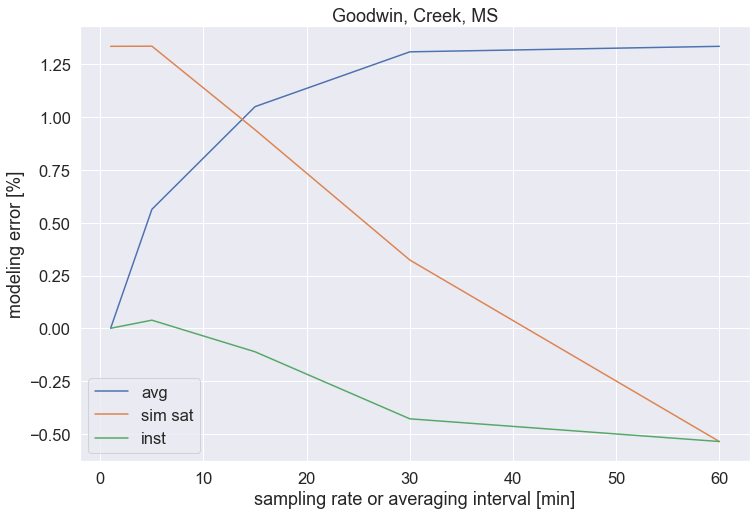
\includegraphics[width=9cm]{analysis/gwn_all.png}}
\caption{Annual AC energy modeling error at Goodwin Creek, MS. There was only one year with sufficient data quality. Time-averaged input (blue) increases with longer averaging interval, simulated satellite (red) decreases with slower sampling rate, while instantaneous (green) is slightly negative from 30 to 60-minutes instantaneous.}
\label{fig:gwn2012}
\end{figure}

\begin{figure}[htbp]
\centerline{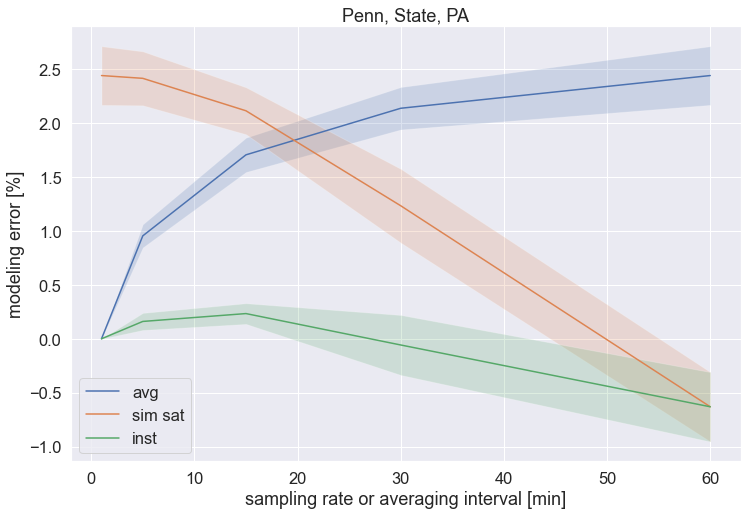
\includegraphics[width=9cm]{analysis/psu_all.png}}
\caption{Annual AC energy modeling error at Penn State, PA. The solid lines and shaded areas show the average and 1-$\sigma$. Time-averaged input (blue) increases with longer averaging interval, simulated satellite (red) decreases with slower sampling rate, while instantaneous (green) is slightly negative at 60-minute instantaneous but relatively unchanged below 30-minutes.}
\label{fig:psu2010}
\end{figure}

\begin{figure}[htbp]
\centerline{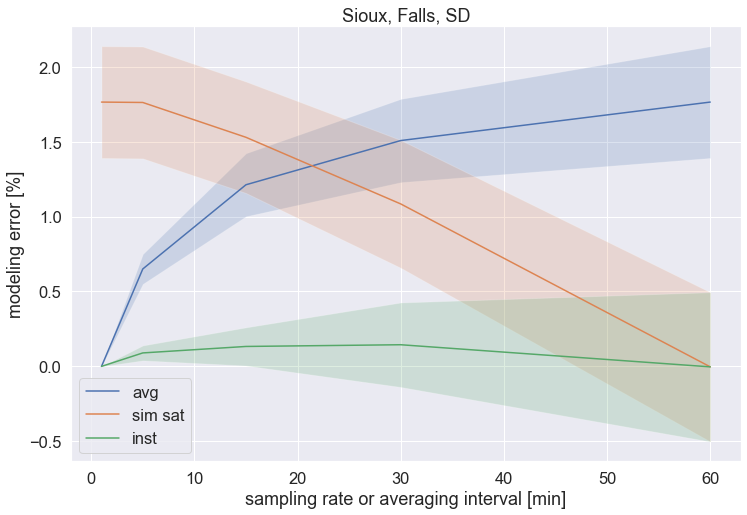
\includegraphics[width=9cm]{analysis/sxf_all.png}}
\caption{Annual AC energy modeling error at Sioux Falls, SD. The solid lines and shaded areas show the average and 1-$\sigma$. Time-averaged input (blue) increases with longer averaging interval, simulated satellite (red) decreases with slower sampling rate, while instantaneous (green) is relatively unchanged.}
\label{fig:sxf2009}
\end{figure}

\begin{figure}[htbp]
\centerline{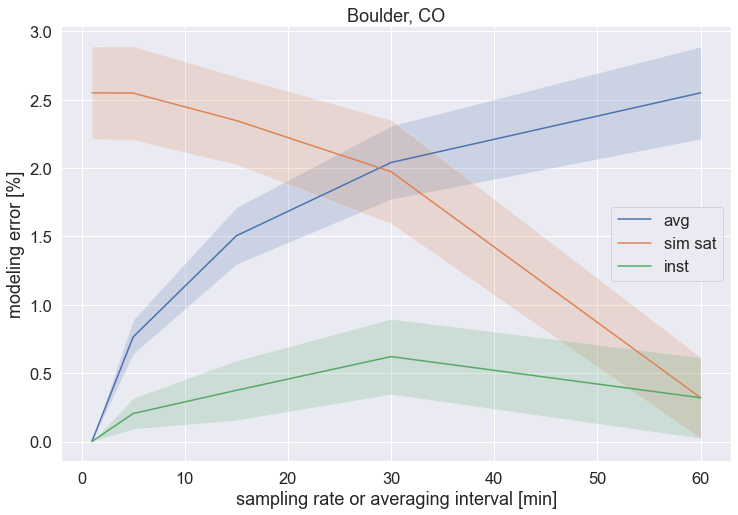
\includegraphics[width=9cm]{analysis/tbl_all.png}}
\caption{Annual AC energy modeling error at Boulder, CO. The solid lines and shaded areas show the average and 1-$\sigma$. Time-averaged input (blue) increases with longer averaging interval, simulated satellite (red) decreases with slower sampling rate, while instantaneous (green) is relatively unchanged.}
\label{fig:tbl2010}
\end{figure}

The largest modeling errors are at Boulder, CO, for both hourly averaged and simulated ``satellite'' at 30-minute sampling rate. Desert Rock, NV, which has the highest annual AC energy output has the lowest modeling errors, which may be affected more by POA irradiance errors than clipping errors due to high irradiance and clear skies. Desert Rock, NV, also has negative modeling errors for instantaneous input sampled every 60-minutes (high-fidelity estimate greater than hourly estimate), which indicates a one-sided distribution at or below the hourly average irradiance, possibly indicating less solar variability and more clear skies. Fort Peck, MT, showed both relatively high modeling errors for hourly average input and slightly negative modeling error for instantaneous input sampled every 60-minutes, perhaps indicating a mixture of cloudy and clear skies. Goodwin Creek, MS, has the second lowest modeling errors yet its annual AC production is similar to Boulder, CO, but only one year was studied, so it may be an outlier. The lowest annual AC output is at Penn State, PA, and it has the 2nd largest modeling error. Bondville, IL, and Sioux Falls, SD, both have fairly large modeling errors similar to Fort Peck, MT. The summary in \ref{table:SURFRAD-summary} shows on average, the modeling error of the simulated ``satellite'' data sampled every 30-minutes, is half that of the hourly averaged input.

\section{Conclusions}
Accurate predictions of energy output are important for decreasing the cost of capital for PV systems, but reports of under-performance for the past few years could damage investor confidence. Modeling errors have been observed when using hourly input data for sites with high solar variability and DC/AC greater than one. However, energy assessments use hourly input from satellite data averaged from coarsely sampled instantaneous measurements with random hourly errors that appear to reduce these modeling errors. We examined the effect of sampling rate on modeling errors by summarizing irradiance data from high frequency ground measurements at the NIST ground array and predicting energy output using SolarFarmer. We repeated this analysis using inputs from the 7 SURFRAD stations and predicted energy output using pvlib python. We observed modeling errors for summarized irradiance input sampled every 30-minutes or shorter averaged hourly as a proxy for satellite, but ignoring spatial effects, and the errors increased for shorter sampling rates. We also observed that when DC/AC ratio is 1.3 or more, clipping errors dominated over other sources like POA irradiance except at sites with high annual energy output. Using high frequency irradiance input at all modeling stages would be ideal, but in practice solar resource data has been pre-summarized hourly, introducing the modeling errors we and others have observed. Therefore, we recommend applying an hourly modeling correction whenever hourly input is used. On average we found this correction can be halved when using satellite data.

\balance
\bibliographystyle{IEEEtran}
% argument is your BibTeX string definitions and bibliography database(s)
\bibliography{IEEEabrv,bibliography}

\end{document}
